%
% File: main.tex (Chapter 2 - Methodology and Experiments)
%
\chapter{Methodology and Experiments}
\label{chap:methodology}
\setlength{\parskip}{1em}

\section{Dataset Description}

We utilize a subset of the Amazon Product Reviews dataset, specifically focusing on the Electronics category with filtering for Headphones-related products. The dataset is sourced from the Stanford SNAP repository \cite{mcauley2015image}.

\subsection{Data Processing}

The following preprocessing steps ensure dataset uniqueness and research reproducibility:
\begin{enumerate}
    \item \textbf{Subcategory Filtering}: Only products categorized under Headphones, Earbuds, or Over-Ear Headphones are retained
    \item \textbf{Implicit Feedback Conversion}: All ratings are converted to binary implicit feedback (1 = interacted)
    \item \textbf{5-Core Filtering}: Users and items with fewer than 5 interactions are iteratively removed
    \item \textbf{Time-Based Split}: Data is split chronologically (70\% train, 15\% validation, 15\% test)
\end{enumerate}

\subsection{Dataset Statistics}

Table \ref{tab:dataset} summarizes the final dataset characteristics after preprocessing.

\begin{table}[H]
\centering
\caption{Dataset Statistics After Processing}
\label{tab:dataset}
\begin{tabular}{ll}
\hline
\textbf{Metric} & \textbf{Value} \\
\hline
Users & 368 \\
Items & 282 \\
Interactions & 2,695 \\
Sparsity & 97.40\% \\
Train Set Size & 1,888 \\
Validation Set Size & 407 \\
Test Set Size & 400 \\
\hline
\end{tabular}
\end{table}

\subsection{Data Distribution Analysis}

Figure \ref{fig:longtail} illustrates the long-tail distribution commonly observed in recommender systems, where a small number of items receive the majority of interactions.

\begin{figure}[H]
\centering
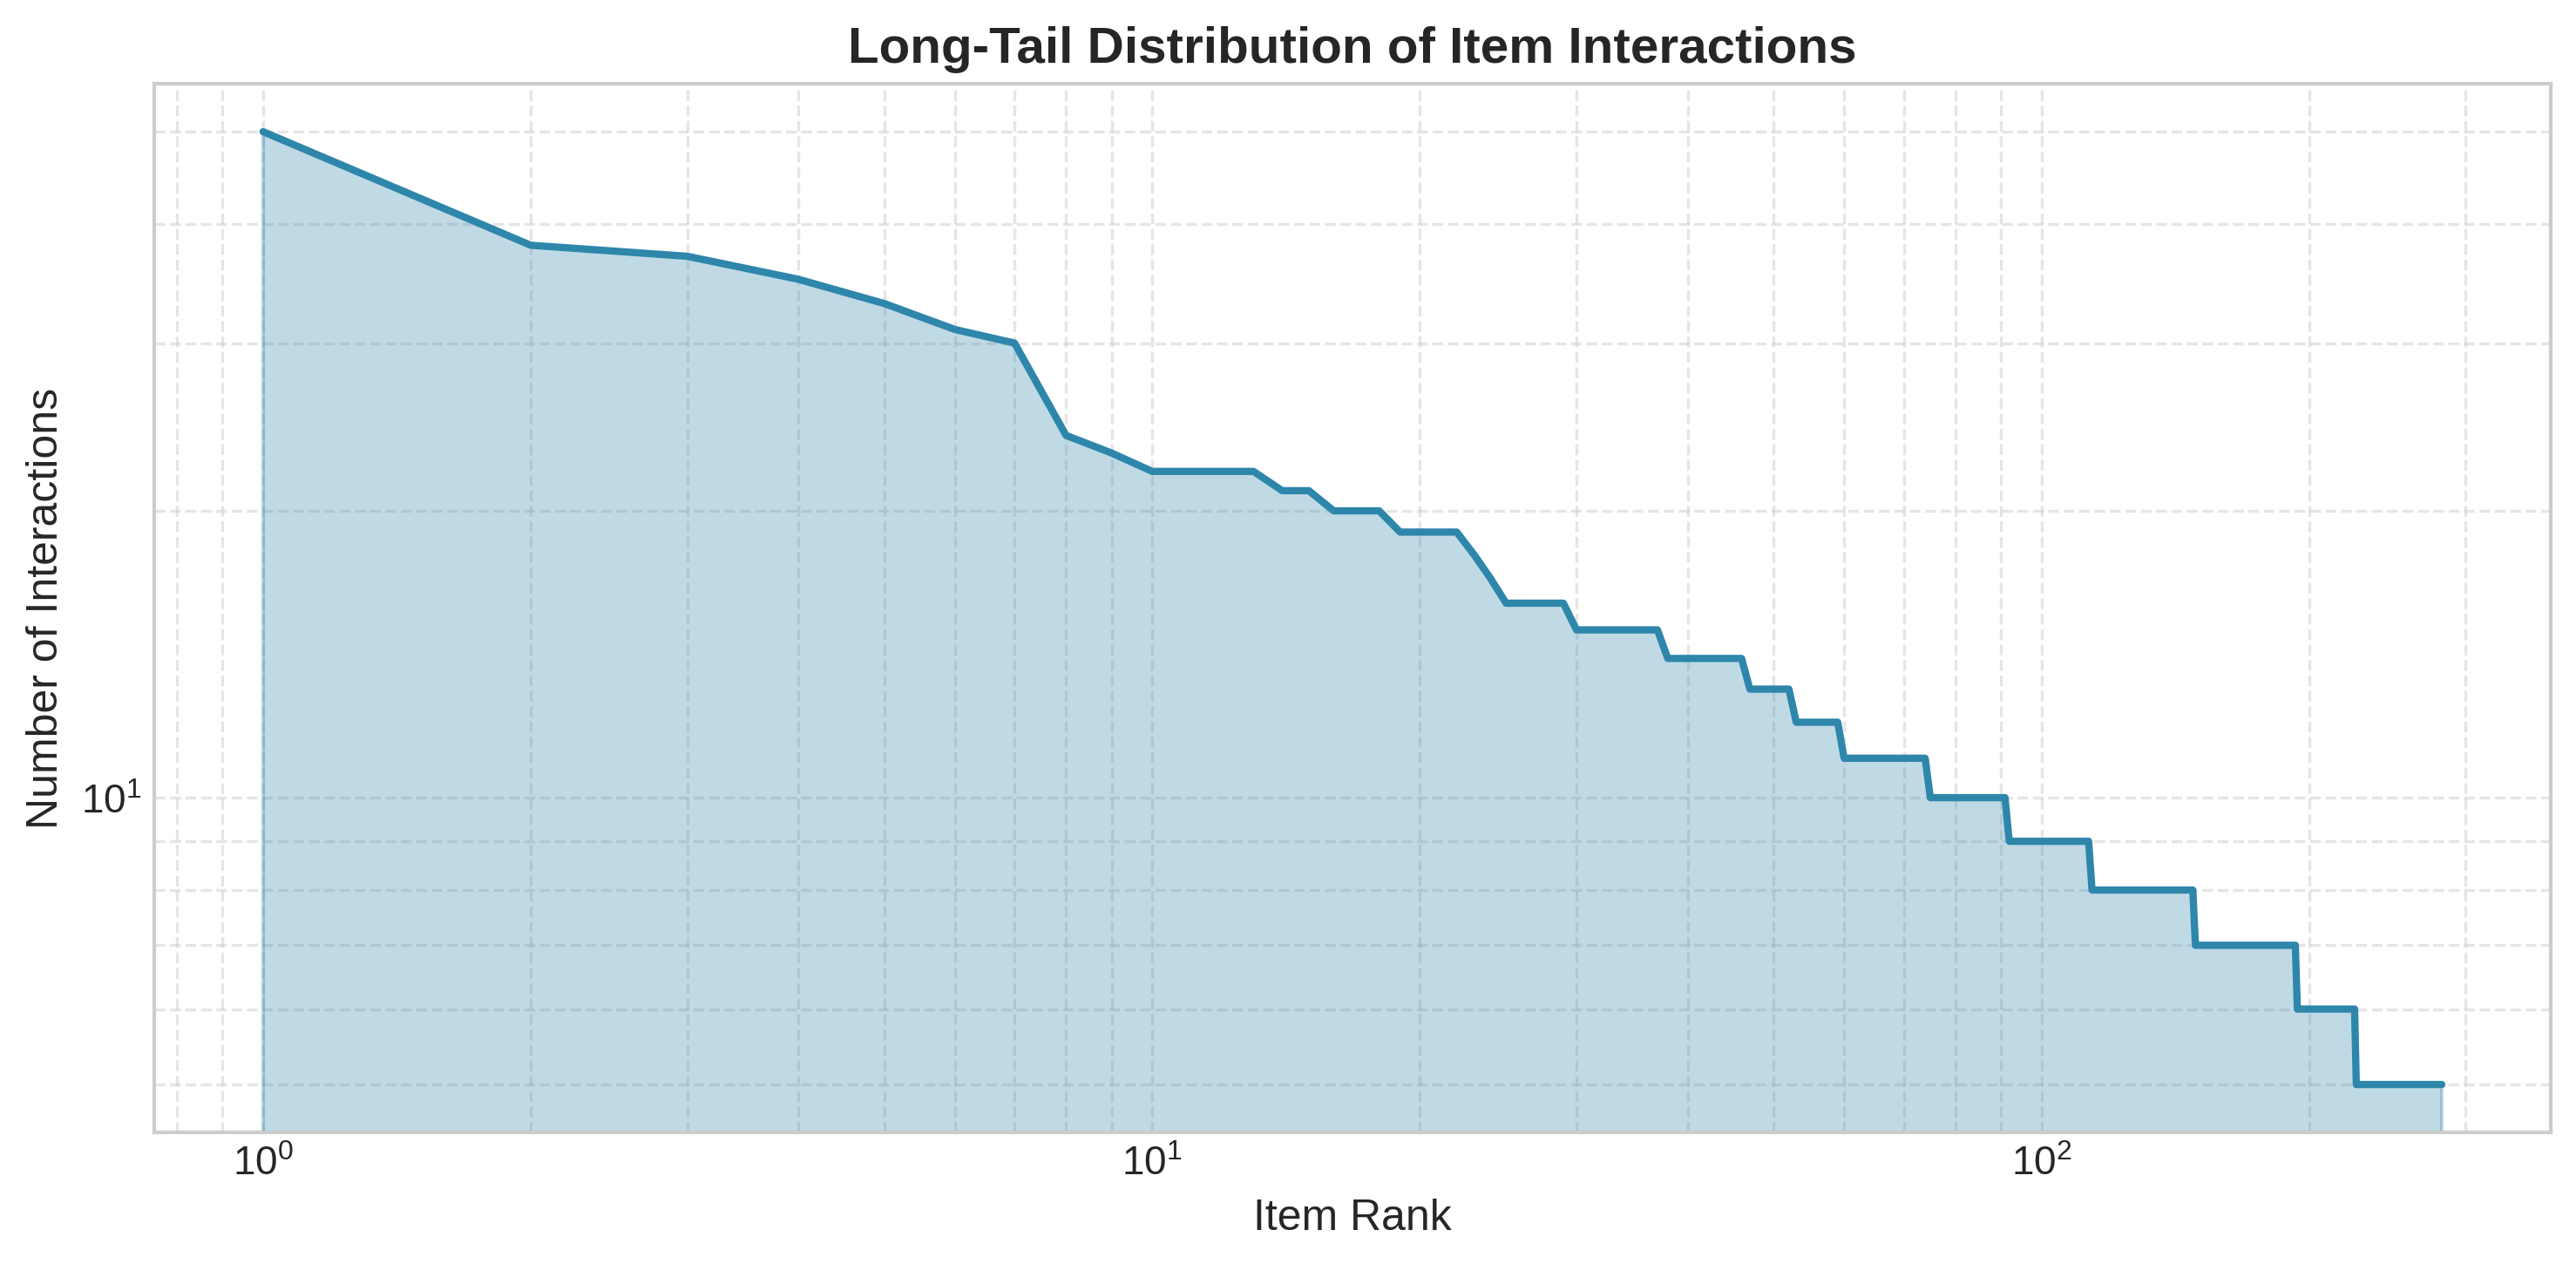
\includegraphics[width=0.8\textwidth]{figures/fig_longtail.png}
\caption{Long-tail distribution of item interactions (log-log scale)}
\label{fig:longtail}
\end{figure}

\section{Problem Formulation}

We formulate the recommendation task as follows:
\begin{itemize}
    \item \textbf{Task}: Top-K Item Recommendation
    \item \textbf{Feedback Type}: Implicit (binary interactions)
    \item \textbf{Output}: Ranked list of items for each user
    \item \textbf{Evaluation}: Ranking metrics (Precision, Recall, NDCG)
\end{itemize}

\section{Models}

\subsection{Popularity Baseline}

The simplest baseline recommends items based on global popularity. For user $u$, the recommendation list consists of the K most frequently interacted items not already seen by $u$.

\subsection{Item-Based Collaborative Filtering}

Item-KNN computes similarity between items based on co-occurrence patterns. Given item $i$ and item $j$, cosine similarity is computed as:
\begin{equation}
    sim(i, j) = \frac{\mathbf{r}_i \cdot \mathbf{r}_j}{||\mathbf{r}_i|| \cdot ||\mathbf{r}_j||}
\end{equation}

\subsection{Matrix Factorization}

Matrix Factorization decomposes the user-item interaction matrix $R$ into low-rank matrices:
\begin{equation}
    \hat{R} = P \cdot Q^T
\end{equation}
where $P \in \mathbb{R}^{|U| \times d}$ and $Q \in \mathbb{R}^{|I| \times d}$ are user and item embedding matrices.

\subsection{Neural Collaborative Filtering (NeuMF)}

NeuMF combines Generalized Matrix Factorization (GMF) with a Multi-Layer Perceptron (MLP) \cite{he2017neural}:
\begin{equation}
    \hat{y}_{ui} = \sigma(h^T(\phi_{GMF} \oplus \phi_{MLP}))
\end{equation}

The architecture consists of:
\begin{itemize}
    \item User and item embeddings for GMF path
    \item User and item embeddings for MLP path
    \item Hidden layers with ReLU activation
    \item Final prediction layer with sigmoid output
\end{itemize}

\section{Evaluation Metrics}

We evaluate using standard ranking metrics:

\textbf{Precision@K}: The fraction of recommended items that are relevant
\begin{equation}
    Precision@K = \frac{|Rec_K \cap Relevant|}{K}
\end{equation}

\textbf{Recall@K}: The fraction of relevant items that are recommended
\begin{equation}
    Recall@K = \frac{|Rec_K \cap Relevant|}{|Relevant|}
\end{equation}

\textbf{NDCG@K}: Normalized Discounted Cumulative Gain
\begin{equation}
    NDCG@K = \frac{DCG@K}{IDCG@K}
\end{equation}

\section{Experimental Setup}

All experiments are conducted with the following configuration:
\begin{itemize}
    \item Embedding dimension: 32
    \item Learning rate: 0.001 (NCF), 0.005 (MF)
    \item Batch size: 256
    \item Negative samples: 4 per positive
    \item Training epochs: 30
    \item Hardware: NVIDIA RTX 2060 GPU
\end{itemize}

\section{Results}

\subsection{Main Results}

Table \ref{tab:results} presents the main experimental results across all models.

\begin{table}[H]
\centering
\caption{Model Performance Comparison}
\label{tab:results}
\begin{tabular}{lcccccc}
\hline
\textbf{Model} & \textbf{P@5} & \textbf{P@10} & \textbf{R@5} & \textbf{R@10} & \textbf{NDCG@5} & \textbf{NDCG@10} \\
\hline
Popularity & 0.0023 & 0.0023 & 0.0043 & 0.0100 & 0.0029 & 0.0050 \\
Item-KNN & 0.0000 & 0.0006 & 0.0000 & 0.0057 & 0.0000 & 0.0020 \\
MF & 0.0011 & 0.0017 & 0.0011 & 0.0054 & 0.0008 & 0.0021 \\
\textbf{NeuMF (NCF)} & \textbf{0.0034} & \textbf{0.0023} & \textbf{0.0071} & \textbf{0.0100} & \textbf{0.0042} & \textbf{0.0059} \\
\hline
\end{tabular}
\end{table}

Figure \ref{fig:comparison} visualizes the model comparison across metrics.

\begin{figure}[H]
\centering

\includegraphics[width=0.95\textwidth]{figures/fig_model_comparison.png}
\caption{Model performance comparison across Precision, Recall, and NDCG@10}
\label{fig:comparison}
\end{figure}

\subsection{Training Dynamics}

Figure \ref{fig:loss} shows the training loss curves for MF and NCF models.

\begin{figure}[H]
\centering

\includegraphics[width=0.8\textwidth]{figures/fig_training_loss.png}
\caption{Training loss over epochs for MF and NCF}
\label{fig:loss}
\end{figure}

\subsection{Cold-Start Analysis}

A significant portion of test users (48.57\%) and items (51.28\%) are "cold" (not seen in training), posing challenges for collaborative filtering approaches.

\begin{figure}[H]
\centering
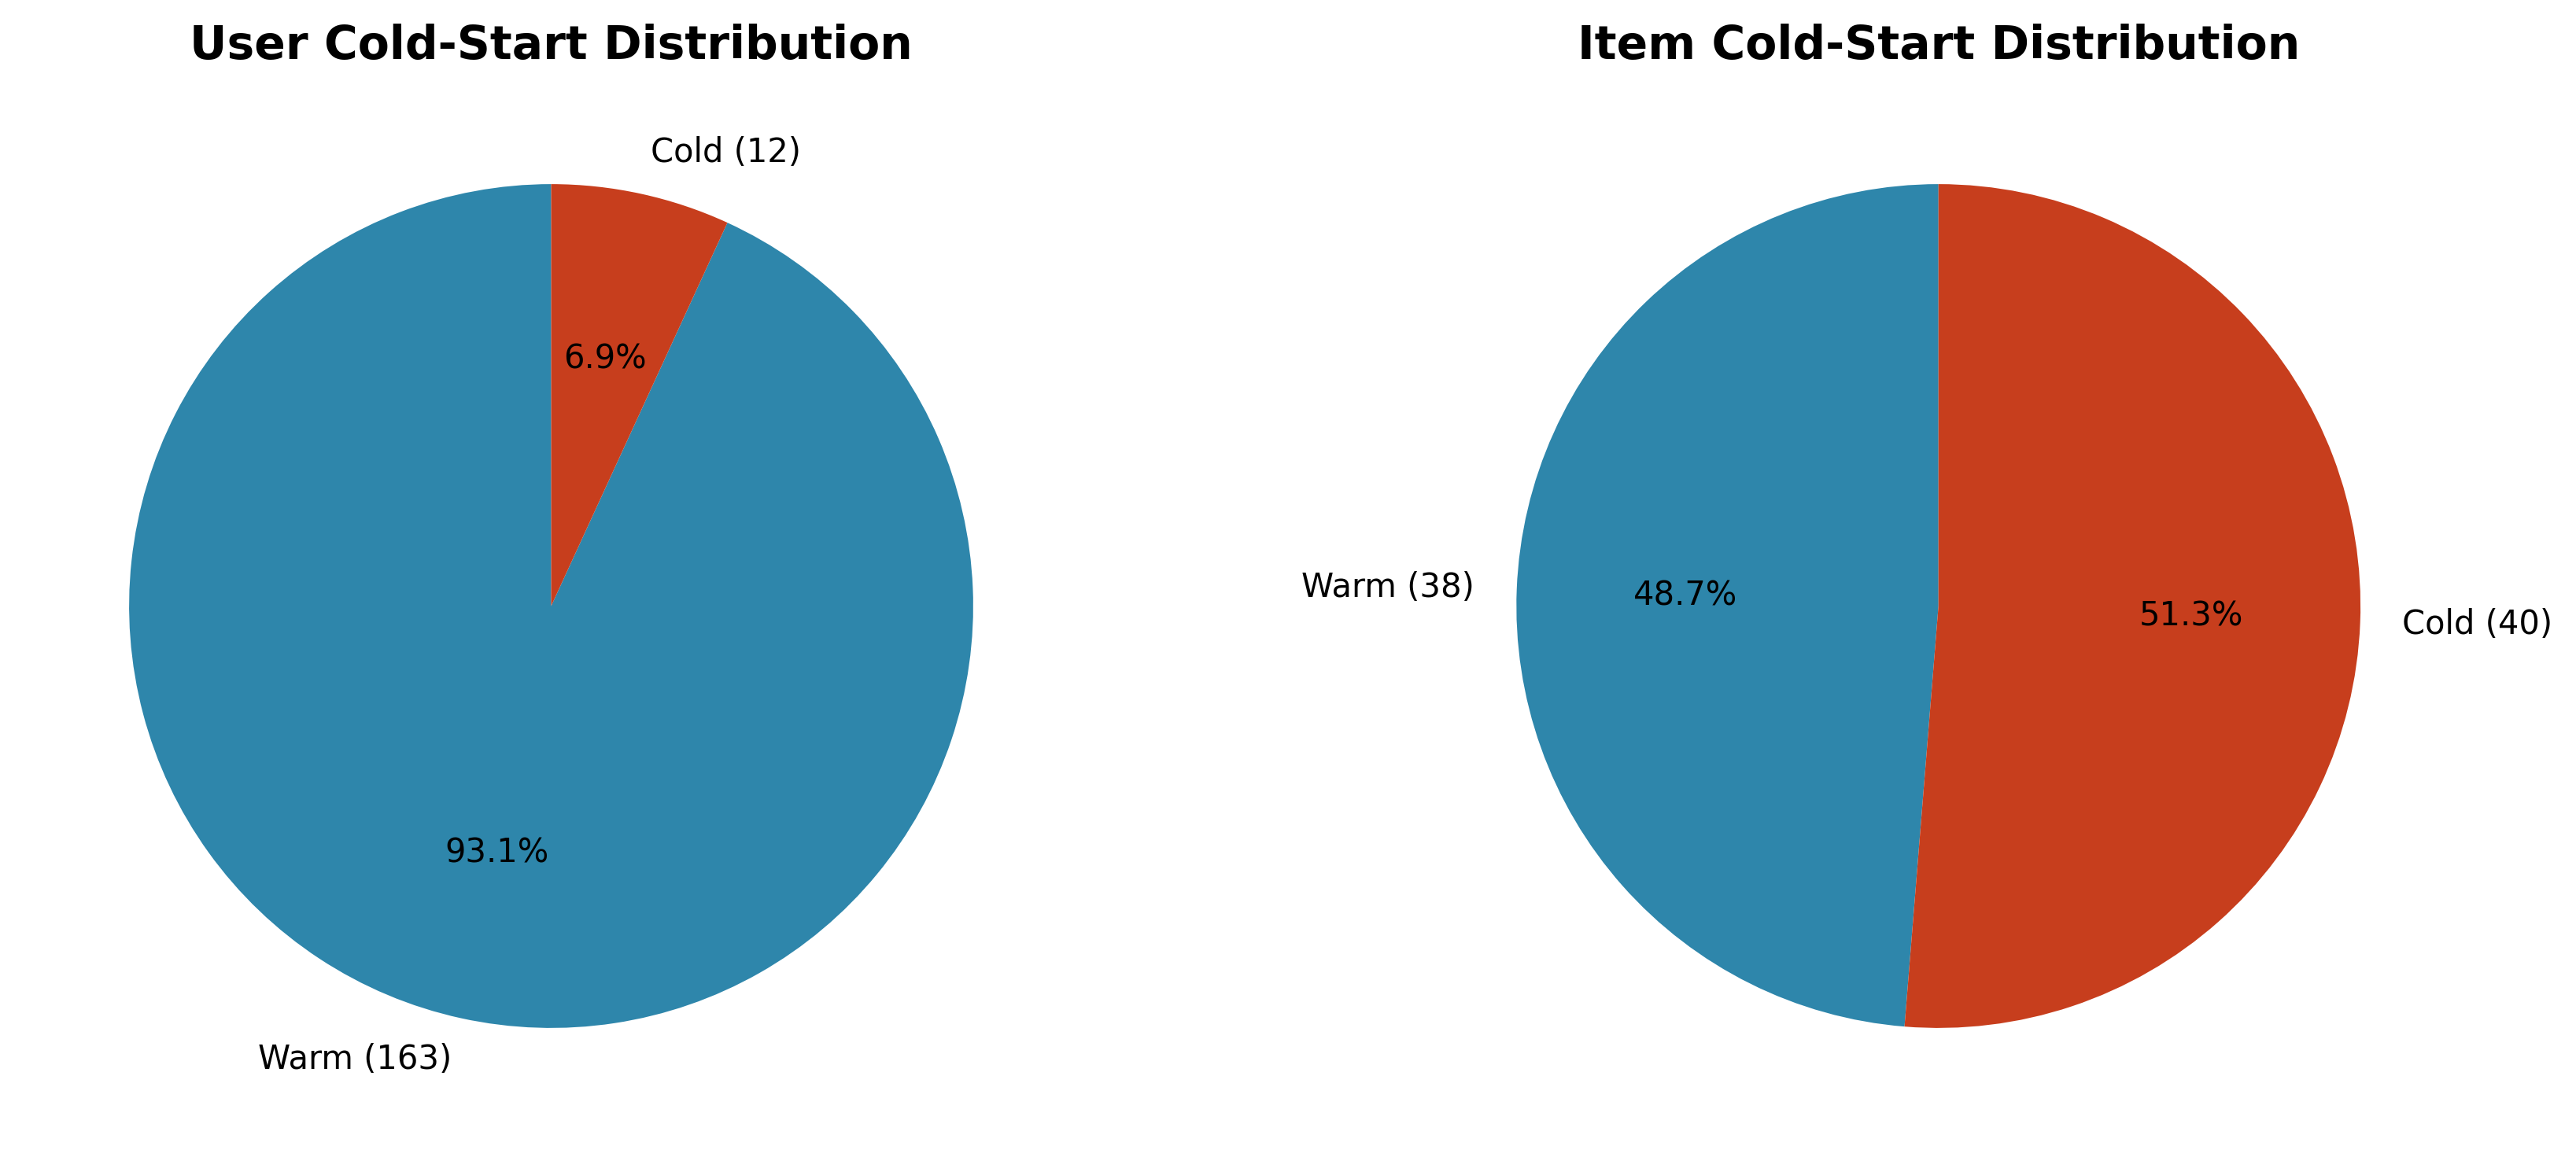
\includegraphics[width=0.8\textwidth]{figures/fig_cold_start.png}
\caption{Cold-start distribution in the test set}
\label{fig:coldstart}
\end{figure}

\section{Discussion}

\textbf{Key Finding 1}: NeuMF achieves the highest NDCG@10 (0.0059), demonstrating that neural architectures can capture complex interaction patterns even in highly sparse settings.

\textbf{Key Finding 2}: The Popularity baseline remains competitive (NDCG@10 = 0.0050), reflecting the strong long-tail effect where popular items dominate.

\textbf{Key Finding 3}: Classical Matrix Factorization underperforms (NDCG@10 = 0.0021), likely due to the extreme sparsity making it difficult to learn meaningful latent factors.

\textbf{Key Finding 4}: Item-KNN shows near-zero performance on Precision@5, indicating that neighborhood-based methods struggle when the interaction matrix is extremely sparse.

\subsection{Model Design Choices}

\textbf{Why not SVD++?} While SVD++ extends basic Matrix Factorization with user and item biases, our experiments with extreme sparsity (97.4\%) suggest that bias terms provide minimal benefit. The limited interaction data makes it difficult to reliably estimate per-user and per-item biases. We therefore opted for the simpler MF formulation to avoid overfitting.

\textbf{Why not LightFM (Hybrid)?} The LightFM library enables hybrid recommendations by incorporating item and user features alongside collaborative signals. However, the Amazon Reviews dataset in our filtered subcategory lacks rich item metadata (e.g., detailed product attributes, brand information). Without meaningful content features, hybrid models reduce to pure collaborative filtering, negating their primary advantage. We acknowledge this as a limitation and suggest that future work with richer metadata could benefit from hybrid approaches.

\subsection{Ablation Study: Embedding Dimension}

We conducted an ablation study to analyze the impact of embedding dimension on model performance. Table \ref{tab:ablation} presents the results for embedding dimensions of 16, 32, 64, and 128.

\begin{table}[H]
\centering
\caption{Ablation Study: Impact of Embedding Dimension on NDCG@10}
\label{tab:ablation}
\begin{tabular}{lcc}
\hline
\textbf{Embedding Dim} & \textbf{MF} & \textbf{NCF} \\
\hline
16 & 0.0063 & 0.0069 \\
32 & 0.0073 & \textbf{0.0119} \\
64 & 0.0057 & 0.0089 \\
128 & 0.0010 & 0.0120 \\
\hline
\end{tabular}
\end{table}

The results indicate that an embedding dimension of 32 provides optimal performance for both models. Lower dimensions (16) lack sufficient representational capacity, while higher dimensions (64, 128) lead to overfitting on the sparse interaction data. This finding is consistent with prior literature suggesting that moderate embedding sizes work best under sparsity constraints.